\documentclass[12pt]{article}

\usepackage[margin=1in]{geometry}  % set the margins to 1in on all sides
\usepackage{graphicx}              % to include figures
\usepackage{amsmath}               % great math stuff
\usepackage{amsfonts}              % for blackboard bold, etc
\usepackage{amsthm}                % better theorem environments
\usepackage{bm}					   % bm for bold math

\usepackage{enumitem} % for [noitemsep]
\usepackage{rotating} % for sideway table
\usepackage{caption} % for newline in caption
\usepackage{xcolor}
\usepackage{hyperref}
\hypersetup{
    colorlinks,
    linkcolor={red!50!black},
    citecolor={blue!50!black},
    urlcolor={blue!80!black}
}
\usepackage{cleveref}

  
\usepackage{float}
\restylefloat{table}

% bibliography
\usepackage{natbib}
\bibpunct{(}{)}{;}{a}{}{,} % no comma between author and year

\title{Two-Sided Matching Model}
\author{Anh Le}

\begin{document}
\maketitle

\section{Using Adaptive Metropolis}

$\alpha$ (length-2 vector) is the employee's preference for the employer's
prestige and autonomy. $\beta$ ($4 \times 18$ matrix) is the employer's
preference for the employee's intercept, age, education, race. There are 18 employers.

I update $\alpha$ and $\beta$ together, using the Adaptive Metropolis algorithm
\citep{Haario2001}. 

The sampling for $\alpha$ and $\beta$ has poor mixing, but does converge towards the same
values (given the same starting points). The values of $\beta$ also make
substantive sense, e.g. professional employer has a positive preference for
education, while farm employer has a negative preference for education.

However, when we start from random, over-dispersed starting points, the mixing
is both extremely poor, and the chains don't converge to any values. 

Below are three MCMC chains from the
same starting points (0 for $\alpha$, and one-sided logit estimates for
$\beta$).

\subsection{3 MCMC chains for $\alpha$}

\begin{figure}[!ht]
\centering
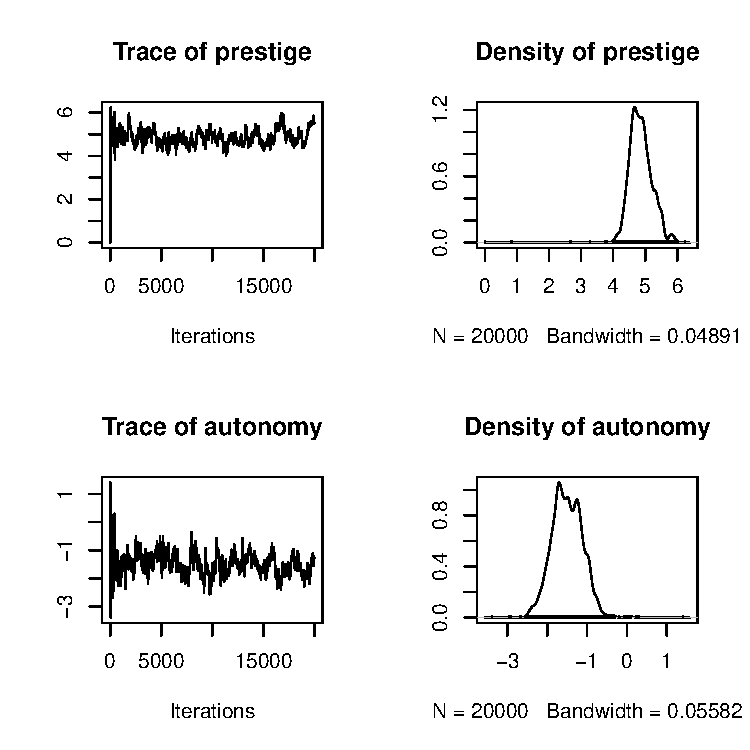
\includegraphics[width=0.8\textwidth]{../figure/trace_alpha_adaptive_replicate1}
\caption{Traceplot of employees' preference for firms' characteristic}
\end{figure}

\begin{figure}[!ht]
\centering
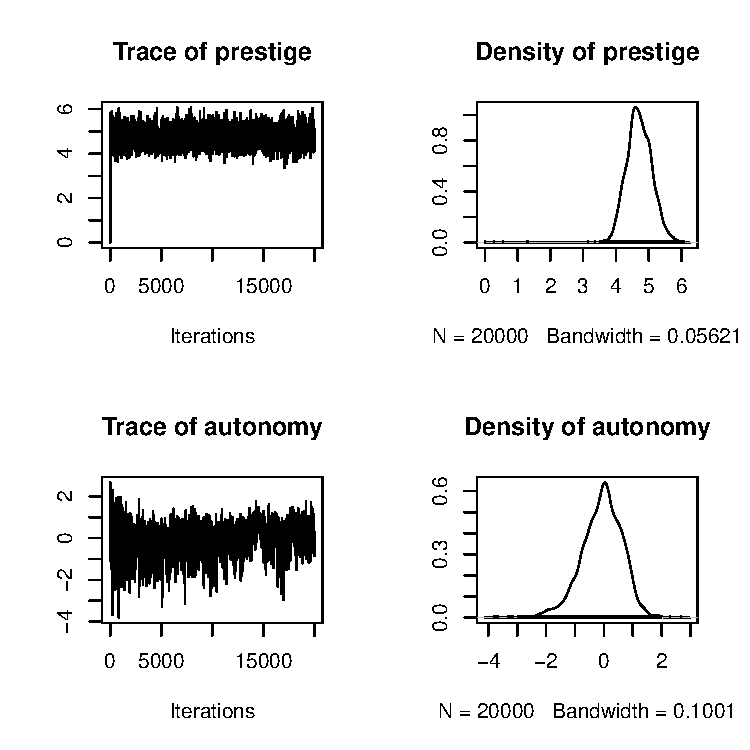
\includegraphics[width=0.8\textwidth]{../figure/trace_alpha_adaptive_replicate2}
\caption{Traceplot of employees' preference for firms' characteristic}
\end{figure}

\begin{figure}[!ht]
\centering
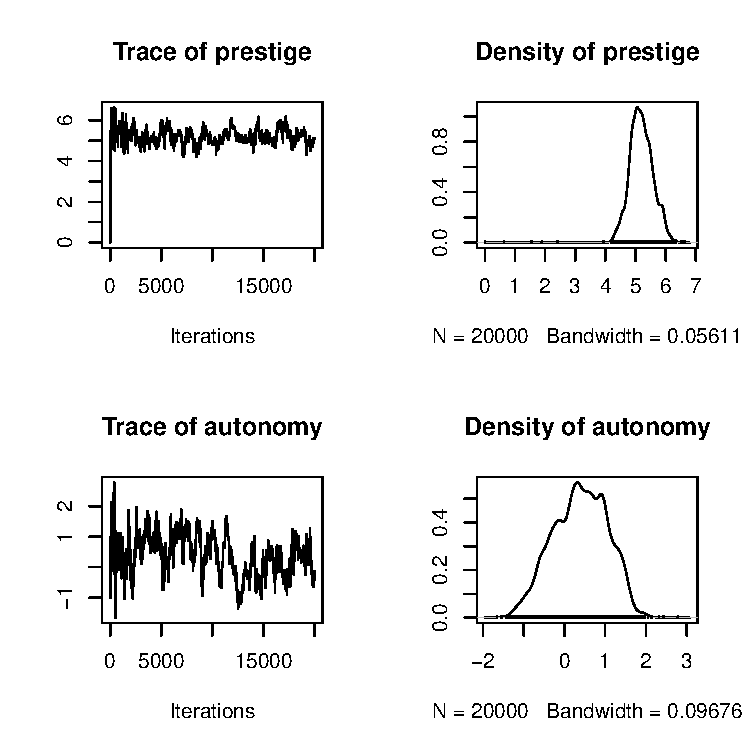
\includegraphics[width=0.8\textwidth]{../figure/trace_alpha_adaptive_replicate3}
\caption{Traceplot of employees' preference for firms' characteristic}
\end{figure}

\subsection{3 MCMC chains for $\beta$}

\begin{figure}[!ht]
\centering
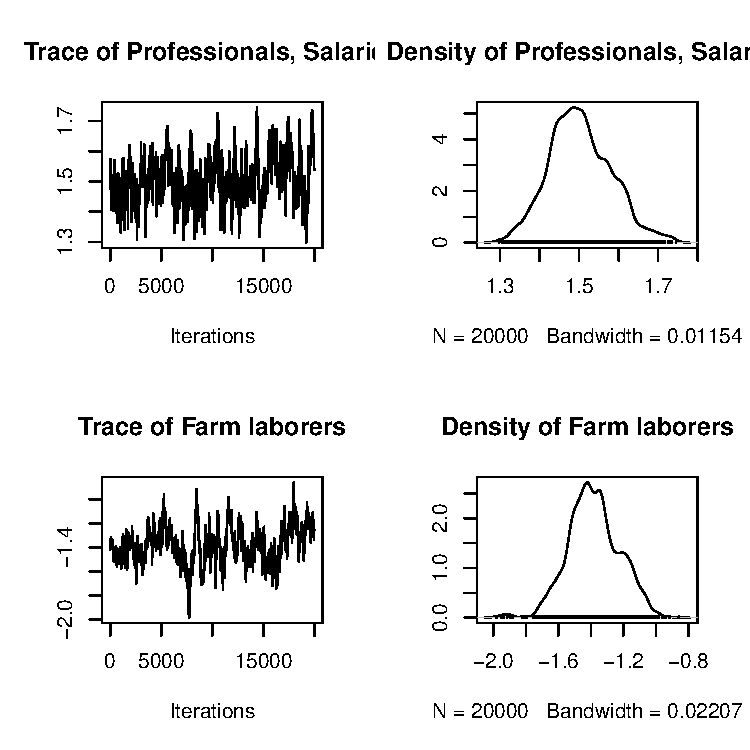
\includegraphics[width=0.8\textwidth]{../figure/trace_beta_adaptive_replicate1}
\caption{Traceplot of employers' preference}
\end{figure}

\begin{figure}[!ht]
\centering
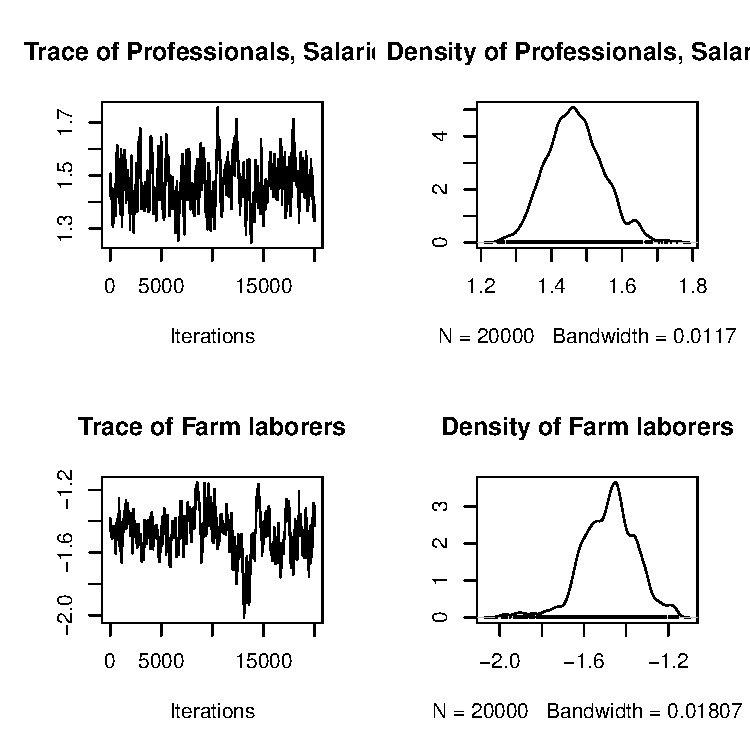
\includegraphics[width=0.8\textwidth]{../figure/trace_beta_adaptive_replicate2}
\caption{Traceplot of employers' preference}
\end{figure}

\begin{figure}[!ht]
\centering
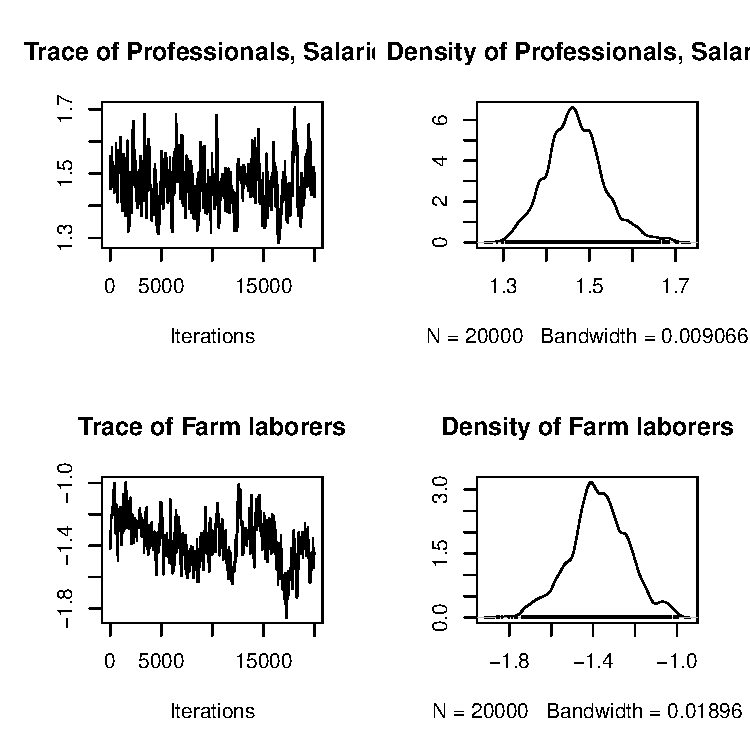
\includegraphics[width=0.8\textwidth]{../figure/trace_beta_adaptive_replicate3}
\caption{Traceplot of employers' preference}
\end{figure}

\subsection{Correlation between $\alpha$ and $\beta$}

To check if the correlation is the cause of slow mixing, I plot the sample
correlation matrix between $\alpha$ and $\beta$. There doesn't seem to be a lot
of correlation

\begin{figure}[!ht]
\centering
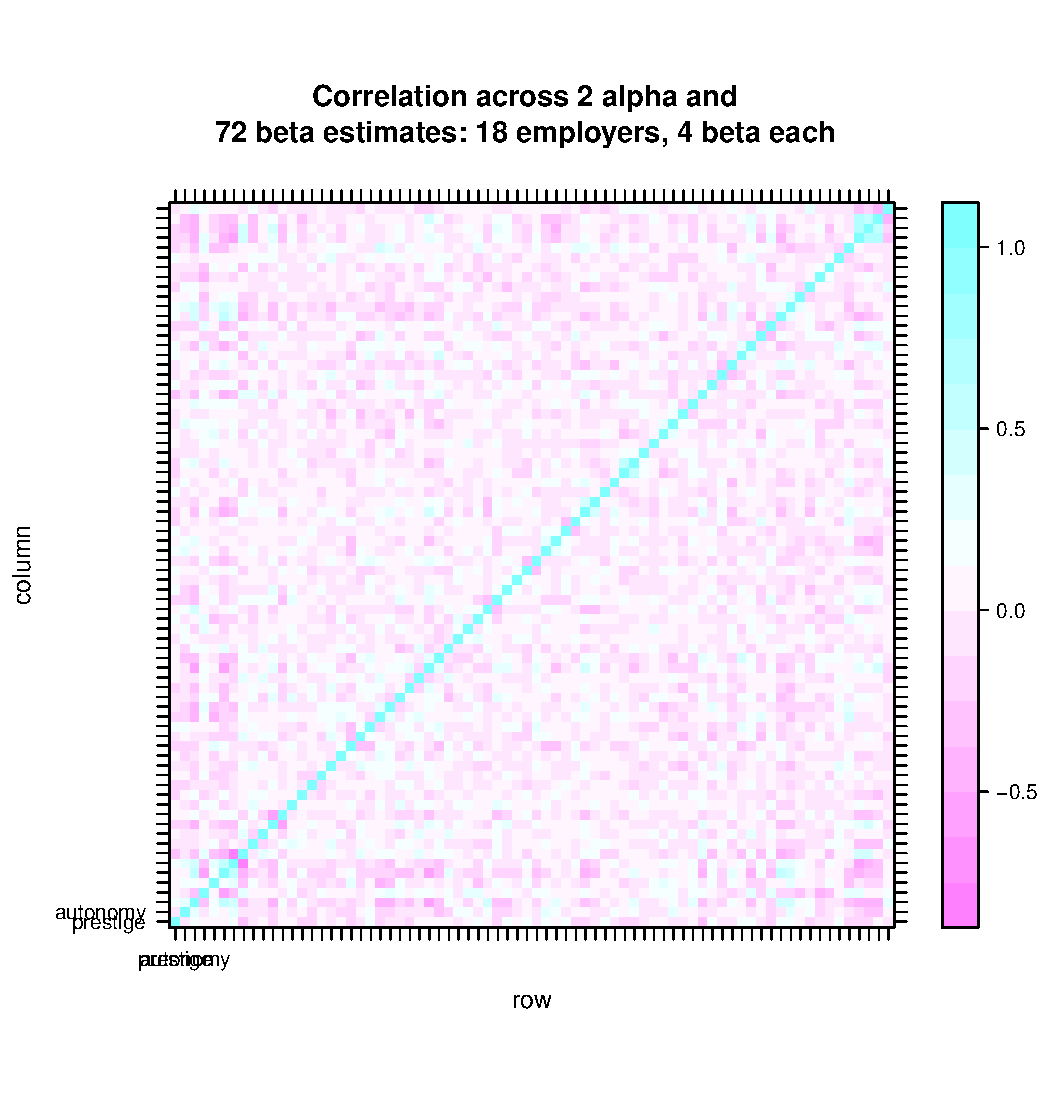
\includegraphics[width=0.8\textwidth]{../figure/correlation_across_alphabeta_adaptive}
\caption{Traceplot of employers' preference}
\end{figure}


\section{Replicating Adaptive Metropolis algorithm}

Replicating the result of \citep{Haario1999, Haario2001}, showing that the
Adaptive Metropolis algorithm outperforms the Metropolis-Hastings (MH) and the
Adaptive Proposal (AP) algorithm. I run each algorithm 100 times, and each
time, record the percentage of the resulting sample that falls within the 68.3\%
confidence region of the target distribution. (Ideally, 68.3\% of the resulting
sample should fall within this region.) The boxplot shows the distribution of
this 100 runs. The boxplot for the Adaptive Metropolis (AM) algorithm is both
closer to the theoretical idea (i.e. horizontal line at 68.3\%) and has a
smaller spread. 


\begin{figure}[!ht]
\centering
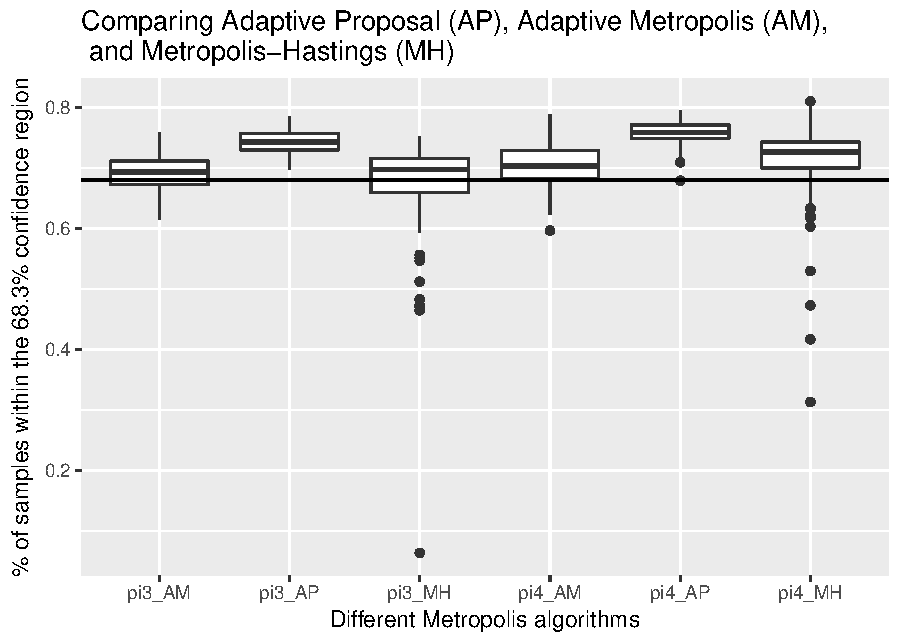
\includegraphics[width=\textwidth]{../figure/comparing_AP_AM_MH}
\caption{Traceplot of employees' preference for firms' characteristic}
\end{figure}

\clearpage
\bibliographystyle{chicago}
\bibliography{library}
\end{document}